\documentclass[11pt]{article}
\usepackage[margin=2.5cm]{geometry}
\usepackage{booktabs}
\usepackage{tabularx}
\usepackage{graphicx}
\usepackage[hidelinks]{hyperref}
\usepackage{times}
\usepackage{enumitem}
\usepackage{float}
\setlist[description]{leftmargin=2.2cm, labelwidth=2.0cm, itemsep=2pt, font=\normalfont\itshape}

\title{Datasets for Subgraph Classification:\\ The Seven Chosen Datasets}
\author{}
\date{October 11, 2026}

\begin{document}
\maketitle

\section*{What we are looking for}

We classify an entity, which we call a \emph{color}, from its subgraph inside one large
graph. In our pregnancy data a node is one visit, a subgraph is all the visits of one patient,
and the label says whether that patient had the outcome. There are $61{,}046$ visits, $6{,}590$
patients and $11\%$ of them positive. Edges join visits with similar text ($20$ neighbours per
visit).

A dataset fits when it has four things. Each node belongs to exactly one subgraph, and a
subgraph has many nodes. There is one label per subgraph, ideally binary. The edges come from
node text or vectors, or are given by the source. And the label cannot be guessed from the size
of the subgraph alone.

Out of the $14$ candidates in the first version of this report, seven were chosen: JODIE
Reddit, Synthea 1k, Synthea 5k, Deezer Europe, CaLiGraph, Amazon, and Gene Ontology with STRING.
This version describes each of them in detail. Three are already built; the other four are not.

\section*{At a glance}

\begin{table}[H]
\centering
\small
\begin{tabularx}{\textwidth}{lXXXl}
\toprule
Dataset & Node & Subgraph (one color) & Label of the subgraph & Status \\
\midrule
Pregnancy (ours) & a visit & a patient's visits & had the outcome & have \\
\addlinespace
JODIE Reddit & a post & a user's posts & user was banned & built \\
Synthea 1k / 5k & a visit & a patient's visits & patient has diabetes & built \\
Deezer Europe & a user & a group of users (to choose) & mostly one gender or not & downloaded \\
CaLiGraph & an entity & the entities of one class & under a parent class or not & not yet \\
Amazon & a product & the products of one category & books or not & not yet \\
GO $+$ STRING & a protein & the proteins of one GO term & under a parent term or not & not yet \\
\bottomrule
\end{tabularx}
\caption{How each dataset is split into subgraphs and what each subgraph is labelled with.
For the last four the grouping and label are our proposal.}
\end{table}

\section*{Disk space}

\begin{table}[H]
\centering
\small
\begin{tabular}{lrrl}
\toprule
Dataset & Download & On disk, unpacked & Source of the number \\
\midrule
JODIE Reddit & $2.3$ GB & $2.3$ GB & measured, already on this PC \\
Synthea 1k & $188$ MB program & $226$ MB & measured, already on this PC \\
Synthea 5k & (same program) & $1.1$ GB & measured, already on this PC \\
Deezer Europe & $2.6$ MB & $7.5$ MB & measured \\
CaLiGraph & $1.4$ GB ($3.8$ GB for all files) & about $10$--$15$ GB & download measured, rest estimated \\
Amazon & $221$ MB & about $1$ GB & download measured, rest estimated \\
GO $+$ STRING & about $200$ MB & about $1$ GB & download measured, rest estimated \\
\midrule
Total & $4.3$ GB & about $16$--$21$ GB & \\
\bottomrule
\end{tabular}
\caption{Space needed for the raw files. Download sizes come from the servers on October 11,
2026. Unpacked sizes for the files not yet downloaded are estimates. The new download is
about $1.8$ GB if JODIE and Synthea, which are already here, are not counted again.}
\end{table}

\paragraph{CaLiGraph is the only large one.} Its files are compressed text that grows about ten
times when unpacked. They can also be read while still compressed, which keeps it at $1.4$ GB.

\paragraph{Built graphs need extra space.} The processed JODIE Reddit graph takes $649$ MB, and
Synthea $130$ MB (1k) and $632$ MB (5k). A processed graph grows with the number of nodes, so
CaLiGraph, with millions of entities, would need many GB unless we keep only part of it.

\section*{The three built datasets}

These numbers come from our own builds.

\begin{table}[H]
\centering
\small
\begin{tabular}{lrrrrrr}
\toprule
 & Subgraphs & Positive & Mean size & Median & Smallest--largest & Size, pos.\ / neg. \\
\midrule
Pregnancy (ours) & $6{,}590$ & $11.4\%$ & $9.3$ & $5$ & $2$--$221$ & $8.3$ / $9.4$ \\
JODIE Reddit & $10{,}000$ & $3.7\%$ & $67.2$ & $44$ & $29$--$4{,}690$ & $61.1$ / $67.5$ \\
Synthea 1k & $1{,}160$ & $14.5\%$ & $58.0$ & $36$ & $1$--$810$ & $\mathbf{166.1}$ / $39.8$ \\
Synthea 5k & $5{,}678$ & $14.6\%$ & $57.4$ & $36$ & $1$--$866$ & $\mathbf{164.8}$ / $39.0$ \\
\bottomrule
\end{tabular}
\caption{Size and label balance of the subgraphs. Size is the number of nodes in a subgraph.
The last column is the mean size of positive and of negative subgraphs.}
\end{table}

\begin{table}[H]
\centering
\small
\begin{tabular}{lrrrr}
\toprule
 & Pieces per subgraph & Edges inside a subgraph & \multicolumn{2}{c}{Same-label neighbours} \\
 & (mean) & (share of all edges) & observed & if random \\
\midrule
Pregnancy (ours) & $8.8$ of $9.3$ nodes & $0.4\%$ & $83.0\%$ & $81.7\%$ \\
JODIE Reddit & $45.9$ of $67.2$ & $10.5\%$ & $93.7\%$ & $93.6\%$ \\
Synthea 1k & $47.7$ of $58.0$ & $5.8\%$ & $79.4\%$ & $51.5\%$ \\
Synthea 5k & $52.5$ of $57.4$ & $2.1\%$ & $79.9\%$ & $51.3\%$ \\
\bottomrule
\end{tabular}
\caption{How the subgraphs sit in the graph. \emph{Pieces} is the number of connected parts of a
subgraph when only its own edges are kept. \emph{Same-label neighbours} looks at edges between
two different subgraphs and asks how often both have the same label; \emph{if random} is what
we would see if those edges were placed at random.}
\end{table}

\paragraph{Our subgraphs are much smaller.} A pregnancy patient has $9$ visits on average. JODIE
and Synthea users and patients have about $60$.

\paragraph{In Synthea the size gives the label away.} Positive patients have about four times
more visits ($165$ against $39$). In JODIE Reddit and in our data both labels have about the
same size.

\paragraph{Subgraphs are not connected inside.} A pregnancy patient with $9.3$ visits falls into
$8.8$ separate pieces. JODIE and Synthea are a bit more connected but still mostly in pieces.

\paragraph{Only Synthea has a label signal in the edges.} In JODIE Reddit and in our data,
neighbouring subgraphs share a label no more often than chance. In Synthea they share it $80\%$
of the time against $51\%$ by chance, which may again come from size.

\begin{figure}[h]
\centering
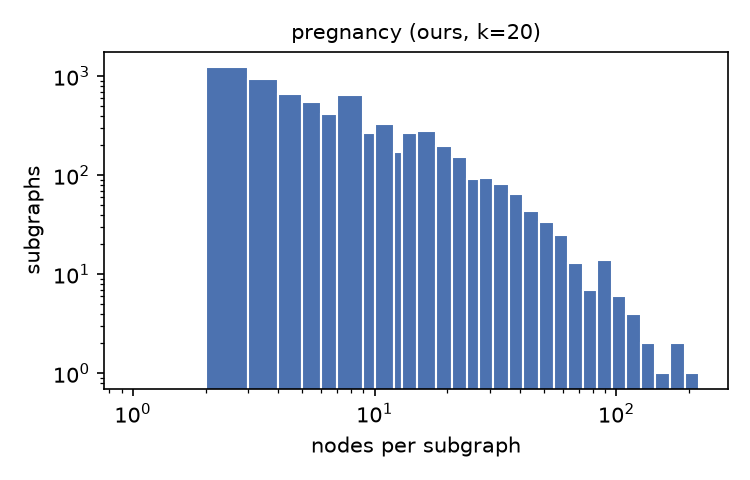
\includegraphics[width=.48\textwidth]{figures/sizes_pregnancy_ours_k_20.png}
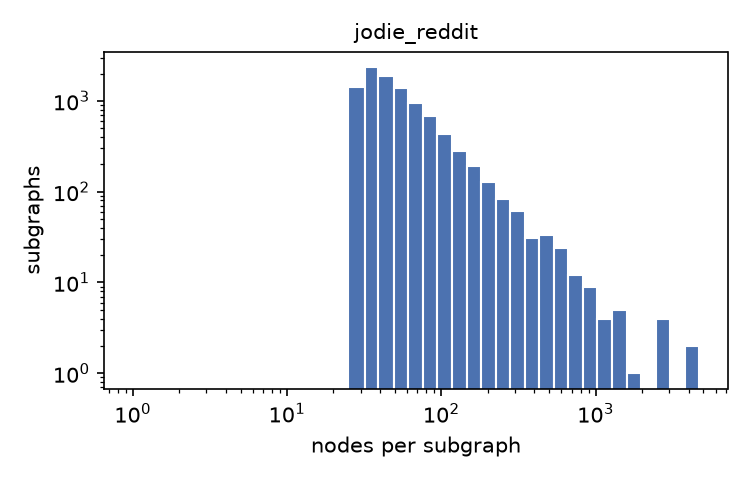
\includegraphics[width=.48\textwidth]{figures/sizes_jodie_reddit.png}\\[4pt]
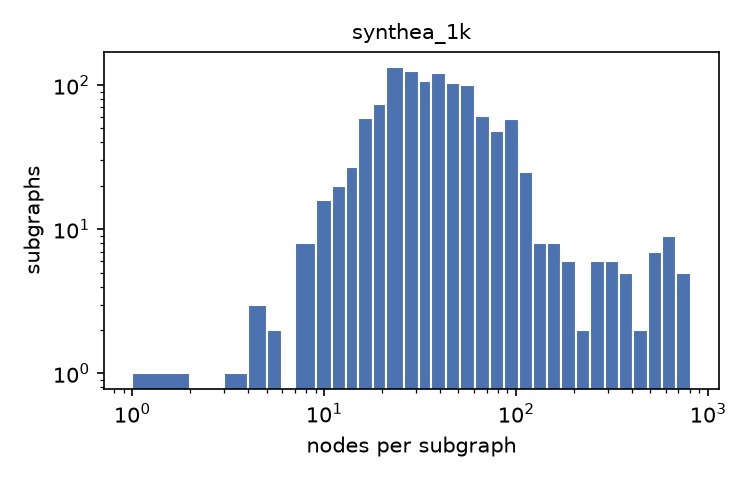
\includegraphics[width=.48\textwidth]{figures/sizes_synthea_1k.png}
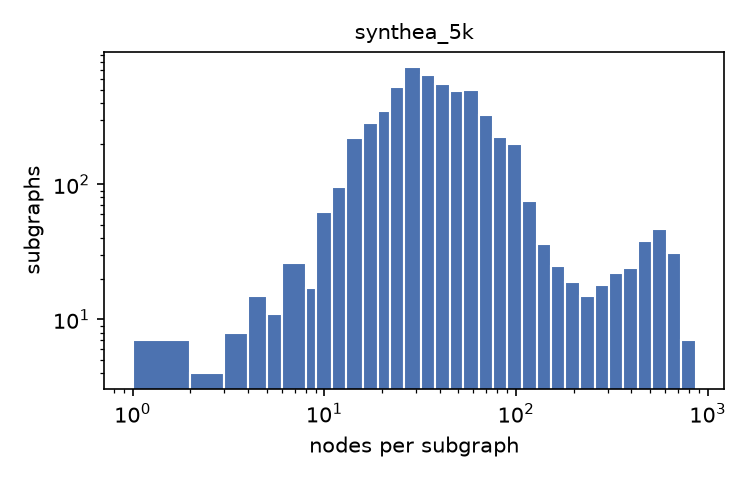
\includegraphics[width=.48\textwidth]{figures/sizes_synthea_5k.png}
\caption{Number of subgraphs of each size, on log axes. Synthea has a second bump of very large
patients, between 200 and 900 visits.}
\end{figure}

\clearpage
\section*{Each dataset in detail}

\subsection*{JODIE Reddit}

From the JODIE paper (Kumar, Zhang and Leskovec, KDD 2019). It records one month of posts by the
$10{,}000$ most active Reddit users in the $984$ most active subreddits (topic forums).

\begin{description}
\item[Source] \href{http://snap.stanford.edu/jodie/reddit.csv}{snap.stanford.edu/jodie}, one
file, \texttt{reddit.csv}, $2.3$ GB. Already in \texttt{data/raw/jodie\_reddit}.
\item[Node] one post. There are $672{,}447$ posts. Each row gives the user, the subreddit, the
time and a ban flag.
\item[Node vector] $172$ numbers made from the post text with LIWC, a tool that counts words by
category (for example sad words or family words). The text itself is not included, so we cannot
embed it our way.
\item[Edges] none are given. We join each post to its $20$ most similar posts by these vectors,
which gives $10.5$ million edges.
\item[Subgraph] all posts of one user. Every user has at least $29$ posts.
\item[Label] $1$ if the user was banned from a subreddit at some point, else $0$. Only $366$
users ($3.7\%$) are positive.
\item[Unused] the subreddit and the time of each post are in the file but not in our graph.
\item[Issues] the label is rare and the LIWC vectors carry little label signal: neighbours share
a label no more often than chance.
\end{description}

\subsection*{Synthea 1k and 5k}

Synthea is a program that makes up realistic medical records (open source, by MITRE). Nothing is
downloaded except the program; the records are generated on our side.

\begin{description}
\item[Source] \href{https://github.com/synthetichealth/synthea}{github.com/synthetichealth/synthea},
one Java file of $188$ MB. Records are made with seed $42$ for $1{,}000$ and $5{,}000$ living
people. People who die along the way are kept too, so we get $1{,}160$ and $5{,}678$ patients.
\item[Files] seven tables per run: patients, encounters (visits), conditions, medications,
procedures, observations (lab tests) and immunizations. Observations is the largest ($145$ MB
of the $226$ MB for 1k).
\item[Node] one visit: $67{,}331$ in 1k and $325{,}760$ in 5k.
\item[Node text] built from the visit: its type and reason, then its diagnoses, procedures,
drugs, vaccines and tests. Every mention of diabetes and its drugs is removed. The text is
embedded with the same small sentence model as before (MiniLM).
\item[Edges] each visit is joined to its $20$ most similar visits by text.
\item[Subgraph] all visits of one patient.
\item[Label] $1$ if the patient has any diabetes condition (prediabetes excluded), else $0$.
About $15\%$ are positive.
\item[Issues] positive patients have four times more visits, so size alone predicts the label.
Synthetic records are also more regular than real ones. A 20k run exists too ($4.5$ GB) but was
not chosen.
\end{description}

\subsection*{Deezer Europe}

A social network of users of the music service Deezer, collected in March 2020 for the FEATHER
paper (Rozemberczki and Sarkar, 2020). We downloaded it to check the files.

\begin{description}
\item[Source] \href{https://snap.stanford.edu/data/feather-deezer-social.html}{SNAP}, one zip of
$2.6$ MB with three files: edges ($1.0$ MB), features ($6.2$ MB) and target ($0.2$ MB).
\item[Node] one user. There are $28{,}281$ users from European countries.
\item[Node vector] the list of artists the user liked, $34$ on average out of $31{,}241$ artists.
Artists are given only as numbers, without names, so there is no text.
\item[Edges] given: $92{,}752$ mutual follows. That is about $6.6$ neighbours per user, against
$32$ in our graph. We could also join users who like the same artists.
\item[Node label] the user's gender, guessed by the authors from the user's name. $44\%$ of users
have label $1$; the files do not say which gender that is.
\item[Subgraph] \textbf{not settled.} The first version proposed the users of one country, but
the files hold no country. A group has to come from the graph itself, for example clusters of
users who follow each other or like the same artists.
\item[Label] $1$ if most users in the group have label $1$, else $0$.
\item[Issues] the subgraph label is made by averaging node labels, so it is only as good as the
name-based gender guess. How many groups we get, and their size, depends on the clustering.
\end{description}

\subsection*{CaLiGraph}

A knowledge graph built from Wikipedia categories and list pages on top of the DBpedia
ontology, by the University of Mannheim (Heist and Paulheim). It has over a million classes and
many millions of entities (people, places, works and so on).

\begin{description}
\item[Source] \href{https://doi.org/10.5281/zenodo.8068322}{Zenodo}, version 3.1.1 of June 2023,
licence CC BY 4.0. The project site, which did not answer on October 10, answered again on
October 11.
\item[Files] $13$ compressed files in N-Triples, a text format with one fact per line, $3.8$ GB
in all. We need four of them, $1.4$ GB: the ontology, which holds the class tree ($32$ MB); the
class of each entity ($525$ MB); the name of each entity ($485$ MB); and the relations between
entities ($345$ MB).
\item[Node] one entity.
\item[Node text] only the entity's name. Longer text, such as the Wikipedia abstract, is not in
these files and would come from DBpedia.
\item[Edges] given: relations between entities, for example a person and the city they were
born in. We could also join entities with similar names or text.
\item[Subgraph] the entities of one class. An entity has many classes, so we keep its most
specific one.
\item[Label] $1$ if the class sits under a chosen parent class (for example Person), else $0$.
\item[Expected] about $10$ entities per class on average, close to our $9$ visits per patient.
\item[Issues] far too large to use whole, so we must cut out a part. Class names and entity names
often say the class outright (``American novelists''), which may make the label easy.
\end{description}

\subsection*{Amazon}

Products sold on Amazon in summer 2006. Two SNAP datasets cover them: a co-purchase graph with
product groups (Yang and Leskovec, 2012) and the product details behind it.

\begin{description}
\item[Source] \href{https://snap.stanford.edu/data/com-Amazon.html}{com-Amazon}: the graph
($4.5$ MB) and its groups ($5.5$ MB).
\href{https://snap.stanford.edu/data/amazon-meta.html}{amazon-meta}: product details,
$211$ MB compressed.
\item[Node] one product. The graph has $334{,}863$ products; the details cover $548{,}552$. That
the two use the same product numbers is likely but not yet checked.
\item[Node text] each product's title and its place in the category tree (for example
Books $>$ Subjects $>$ History). Reviews give date, star rating and votes, but \textbf{no review
text}; the first version of this report was wrong on this point.
\item[Edges] given: $925{,}872$ pairs of products often bought together. We could also join
products with similar titles.
\item[Subgraph] the products of one category. SNAP already splits each category into its
connected parts and drops parts under $3$ products. A product can sit in several categories, so
we keep one.
\item[Label] $1$ if the category holds books, else $0$. Books are $72\%$ of products
($393{,}561$), then music ($103{,}144$), videos ($26{,}132$) and DVDs ($19{,}828$). High against
low average rating is an alternative label.
\item[Issues] the book label is unbalanced the other way (most are positive), and the title and
category path may give it away.
\end{description}

\subsection*{Gene Ontology and STRING}

Human proteins. STRING gives which proteins work together; Gene Ontology (GO) gives what each
protein does, as terms arranged in a tree. SubGNN's PPI-BP dataset is built the same way:
$21{,}521$ proteins, $1{,}591$ subgraphs of about $10$ proteins each, and $6$ classes.

\begin{description}
\item[Source] \href{https://version-12-0.string-db.org/cgi/download?species_text=Homo+sapiens}{STRING v12}
for human: links ($79$ MB), protein info ($2$ MB), names in other databases ($19$ MB), and two
ready-made sets of protein vectors ($19$ and $36$ MB).
\href{https://geneontology.org/docs/download-go-annotations/downloads/}{GO}: the human
annotation file ($12$ MB) and the term tree ($32$ MB). About $200$ MB in all.
\item[Node] one protein, about $19{,}000$ in STRING (from memory).
\item[Node text] a short description of each protein in the STRING info file. STRING also gives
vectors made from the protein sequence and from the network.
\item[Edges] given: pairs of proteins with a confidence score from $0$ to $1000$. We keep pairs
above a cut-off, for example $700$ (high confidence).
\item[Matching] STRING uses its own protein ids and GO uses UniProt ids. The STRING names file
maps one to the other.
\item[Subgraph] the proteins of one GO term. A protein has many terms, so we keep one, or allow
overlap.
\item[Label] $1$ if the term sits under a chosen branch of the GO tree, else $0$.
\item[Issues] the protein descriptions often state the function, which is close to the label.
Some GO terms are themselves inferred from the same kind of evidence as STRING edges.
\end{description}

\end{document}
